



\lstset{language=R}
\begin{lstlisting}
library(raster)
library(rasterVis)
library(maptools)
library(latticeExtra)
library(colorspace)
\end{lstlisting}


\lstset{language=R}
\begin{lstlisting}
old <- setwd(tempdir())
download.file('http://www.gadm.org/data/shp/BRA_adm.zip', 'BRA_adm.zip')
unzip('BRA_adm.zip')
download.file('http://www.diva-gis.org/data/msk_alt/BRA_msk_alt.zip', 'BRA_msk_alt.zip')
unzip('BRA_msk_alt.zip')
download.file('http://www.diva-gis.org/data/alt/BRA_alt.zip', 'BRA_alt.zip')
unzip('BRA_alt.zip')
download.file('http://www.diva-gis.org/data/wat/BRA_wat.zip', 'BRA_wat.zip')
unzip('BRA_wat.zip')


proj <- CRS(' +proj=longlat +ellps=WGS84')
brazilAdm <- readShapePoly('BRA_adm1.shp', proj4string=proj)
Encoding(levels(brazilAdm$NAME_1)) <- 'latin1'
centroids <- coordinates(brazilAdm)
xyBrazil <- apply(centroids, 2, mean)

brazilWat <- readShapeLines('BRA_water_lines_dcw.shp', proj4string=proj)
Encoding(levels(brazilWat$NAM)) <- 'latin1'
brazilAlt <- raster('BRA_alt')
brazilMskAlt <- raster('BRA_msk_alt')
brazilWatArea <- readShapePoly('BRA_water_areas_dcw.shp', proj4string=proj)

setwd(old)
\end{lstlisting}




\lstset{language=R}
\begin{lstlisting}
river <- subset(brazilWat,
                subset=brazilWat$HYC_DESCRI=='Perennial/Permanent' & brazilWat$NAM!='UNK')
\end{lstlisting}


\lstset{language=R}
\begin{lstlisting}
## Quizas mejor usar pointLabel para sp cuando Roger la incorpore
## a maptools. Asi mejoran los solapes. Y mejor romper los
## strings con saltos de linea de forma externa a la funcion.
panel.labels <- function(x, y=NULL, labels,
                         gp=gpar(cex=0.7, col='black',
                           fontfamily='Palatino', lineheight=.8,
                           fill='lightgray', alpha=0.7))
{
  xy <- xy.coords(x, y)


  widthOriginal <-  sapply(labels, function(s){
    tg <- textGrob(s, gp=gp)
    gw <- grobWidth(tg);
    convertWidth(gw, 'native', valueOnly=TRUE)
  })

  heightOriginal <-  sapply(labels, function(s){
    tg <- textGrob(s, gp=gp)
    gh <- grobHeight(tg);
    convertHeight(gh, 'native', valueOnly=TRUE)
  })

  rg <- rectGrob(x=xy$x, y=xy$y,
                 width=widthOriginal, height=heightOriginal,
                 default.units='native',
                 gp=gpar(fill=gp$fill, col='transparent', alpha=gp$alpha))
  grid.draw(rg)

  tg <- textGrob(x=xy$x, y=xy$y, label=labels,
                 default.units='native',
                 gp=gp)
  grid.draw(tg)
}
\end{lstlisting}


\lstset{language=R}
\begin{lstlisting}
admNames <- strsplit(as.character(brazilAdm$NAME_1), ' ')

admNames <- sapply(admNames,
                 FUN=function(s){
                   sep=if (length(s)>2) '\n' else  ' '
                   paste(s, collapse=sep)
                   })
\end{lstlisting}


\lstset{language=R}
\begin{lstlisting}
terrainTheme <- rasterTheme(region=terrain_hcl(15))
terrainTheme$panel.background$col = 'skyblue3'

levelplot(brazilAlt, par.settings=terrainTheme) +
  layer(sp.polygons(brazilAdm, col='black', lwd=0.6)) +
  layer(sp.lines(river, col='skyblue3', lwd=0.8)) +
  layer(sp.polygons(brazilWatArea, col='darkblue', fill='blue')) +
  layer(sp.pointLabel(centroids, labels=admNames,
                       cex = 0.8, fontfamily = 'Palatino')) +
  layer(panel.text(xyBrazil[1], xyBrazil[2], labels='BRAZIL',
                   cex=2, fontfamily = 'Palatino'))
\end{lstlisting}

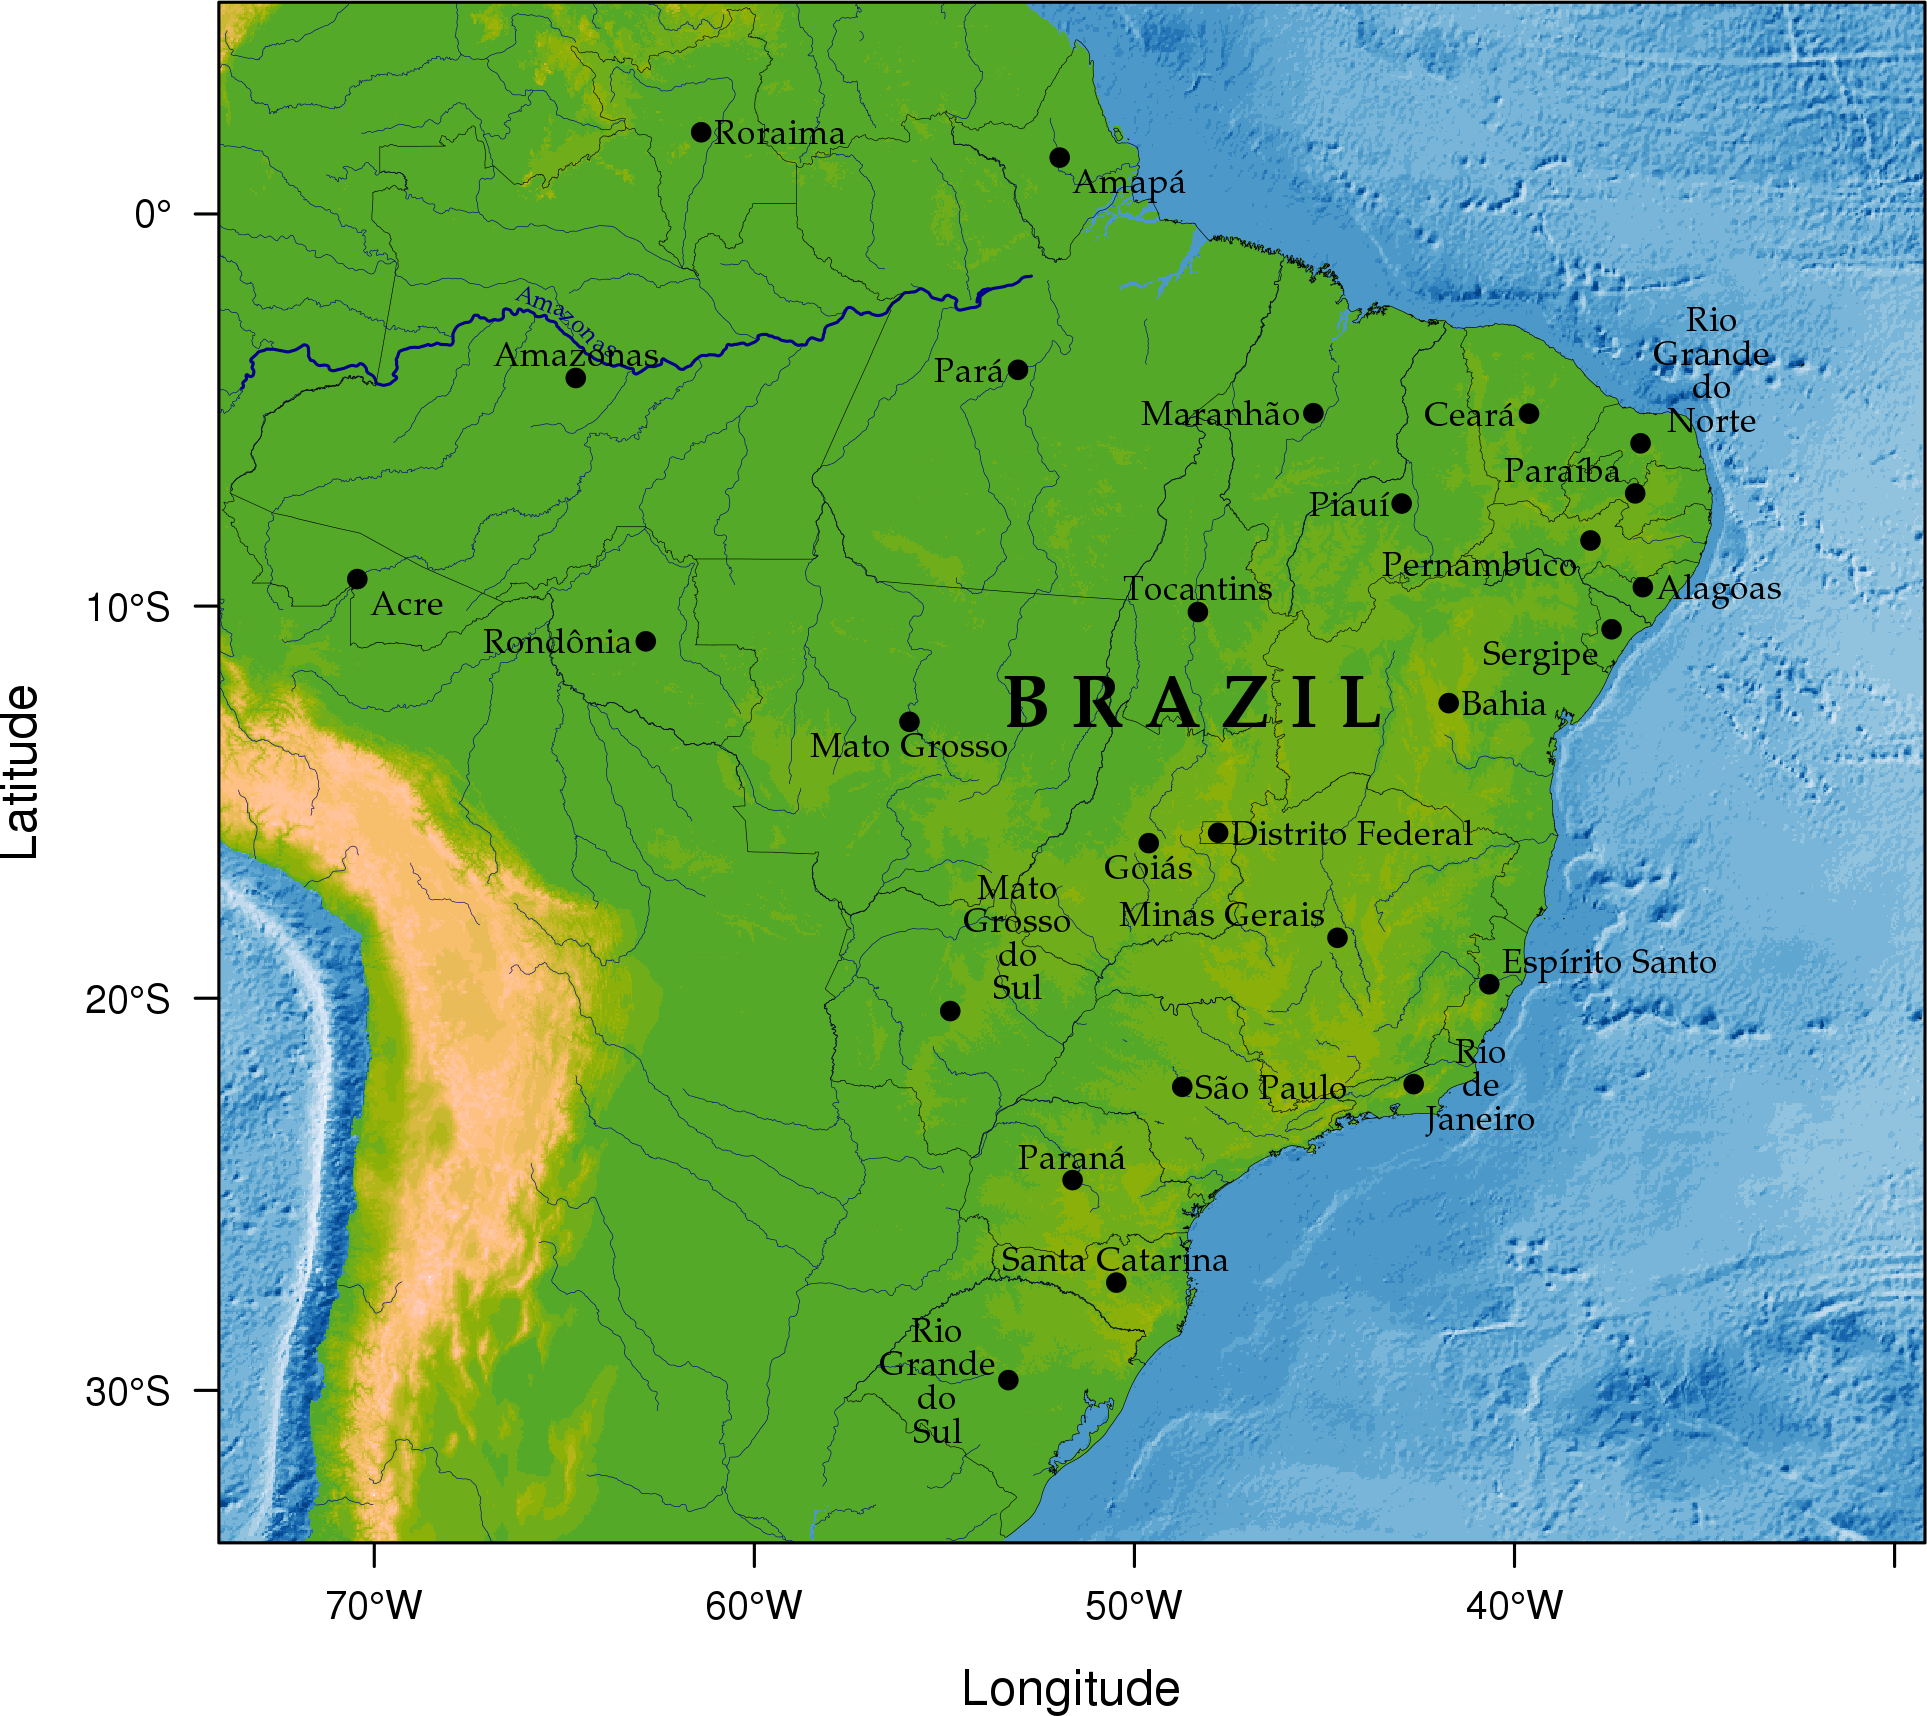
\includegraphics[width=.9\linewidth]{figs/brazil.pdf}

